\documentclass[12pt,a4paper]{article}
\usepackage[utf8]{inputenc}
\usepackage[T1]{fontenc}
\usepackage{amsmath}
\usepackage{amsfonts}
\usepackage{amssymb}
\usepackage{graphicx}
\usepackage{harvard}
\usepackage{mathptmx}
\usepackage{setspace}
\author{Waseem Syed}






\title{Artificial Intelligence Coursework}
\date{}

\begin{document}
	\maketitle
	
	
	\section{Reinforcement Learning}
	
	{\setstretch{1.5}
	Select a single topic from Search Techniques, Deep Learning and Reinforcement Learning, and write a brief literature review report on it.  You may make use of materials which you find in the lecture notes, textbooks and the Internet, but you should adapt them to your report and give full citations and references to sources each time copied material is used (8 marks).  The main aim of the report is to provide your understanding, critical analysis and evaluation of the selected topic in terms of observations and/or application examples (12 marks). The report should be 3 pages using Times New Roman Font, 12 point, with 1.5 spacing, including references and Web/Book citations. Longer submissions will not be penalized but will not necessarily draw extra credit. {20 marks}\\
	\\
	\\
	

\cite{sutton2011reinforcement} says that the term 'reinforcement learning' is used to denote a more general approach, so that an action applied to the environment in a particular state produces an immediate reward and a change of state. The long-term return from the action is sum of the immediate reward and the return achievable from the new state. The return obtainable from the each state, or 'value' of the state, is therefore evaluated by a form of bootstrapping, since the value of any one state depends on the values of others that can be reached from it.
	
}
	
		\bibliographystyle{agsm}
	\bibliography{bibliography}
	
	
	\section{Question}
	Write a research essay/report on temporal logics and/or their application in the domain of Artificial Intelligence. It can be about any relevant theoretical and / or practical topics, such as:
	
		\begin{itemize}
		
	
    \item Time Theories and / or Models
	\item Temporal Knowledge Representation and Management
	 \item  Temporal Data Mining or Case-Based Reasoning
	 \item  Time Series and / or State Sequences
	  \item Temporal Database Management
	\item  Reasoning about action, event and change
	 \item Prediction / Planning
	\item  Diagnosis / Explanation
	\item Industrial Process Control
    \item Historical Reconstruction
	\item Natural Language Understanding
\end{itemize}
	etc., but only focusing on a SINGLE topic. You may make use of materials which you find in the lecture notes, textbooks and the Internet, but you should adapt them to your essay and give full citations and references to sources each time copied material is used. The contents of the essay/report must be related to the key words “Time” and/or “temporal”, in terms of a well-presented literature review/survey (8 marks), together with your own understanding, observations, critical analysis and evaluation of temporal logics and/or their applications in the domain of Artificial Intelligence (12 marks). The essay/report should be around 5 pages using Times New Roman Font, 12 point, with 1.5 spacing, including references and Web/Book citations. Longer submissions will not be penalized but will not necessarily draw extra credit.{20 marks}
	
	
	
	\section{Question} 
	Assume that the universe of discourse is the set of people studying or working at the University of Greenwich. Rewrite the following statements in the form of predicate logic.
		\subsection{(a)}
		Each person is either a student or a staff.
		
	$\forall$x(student(x)$\lor$staff(x))
		
		
		
		\subsection{(b)}
		Each lecturer teaches some modules.	\\
		$\forall$ x $\exists$y(lecturer(x)$\rightarrow$teaches(x,y)$\wedge$ module(y))
		
		
		
		
		
		\subsection{(c)}
		Some hard-working people are not boring.\\
		$\exists$x(hard-working people(x) $\wedge$ $\mathord{\sim}$boring(x))
		
		
		
		
		
		\subsection{(d)}
		Hard-working people are respectable.\\
		
		
		
		$\forall$ x(hard-working people(x) $\rightarrow$ respectable(x)\\
	
		
		
		
		\subsection{(e)}
		Everyone knows some hard-working people.\\
	    $\forall$x 	$\exists$y(hard-working(y)$\wedge$knows(x,y)))
		
		
		
	\section{Question}
		\subsection{(a)}
	
		Use a truth table to verify the following equivalence:
		
		
			A $\wedge$ B $\rightarrow$ C $\equiv$ $\mathord{\sim}$ A $\lor$ $\mathord{\sim}$ B $\lor$ C
		
	
				
			
				
	
			\begin{tabular} {|l|l|l||l|l|l||l|l||l|}
				\hline
				\hline
				A&B&C& $\mathord{\sim}$  A&$\mathord{\sim}$ B& A $\wedge$ B& $\mathord{\sim}$ A $\lor$ $\mathord{\sim}$ B& A $\wedge$ B $\rightarrow$ C& $\mathord{\sim}$ A $\lor$ $\mathord{\sim}$ B $\lor$ C \\
				\hline
				\hline
			T&T&T&F&F&T&F&T&T \\
			
			T&T&F&F&F&T&F&F&F \\
			T&F&T&F&T&F&T&T&T \\
			T&F&F&F&T&F&T&T&T \\
			F&T&T&T&F&F&T&T&T \\
			F&T&F&T&F&F&T&T&T \\
			F&F&T&T&T&F&T&T&T \\
			F&F&F&T&T&F&T&T&T\\
			\hline
				
			\end{tabular}
			
	
		
		
	\newpage
			
			
	\subsection{b}
		List the four main representation schemas learnt from this course and give a typical 	example for each of them.
		\begin{itemize}
			
		\item[1] Logic Representation:\\
		Typical examples of logical representation are Predicate Logic and Propositional logic.
		
		
		\item[2] Procedural Representation:\\
		Production systems are a typical example of procedural representations.A production system has three components:\\
		A database of facts (also called data memories, or working memories)\\	
		A set of production rules (also called condition-action rules, or production memory)\\	
		An interpreter (also called inference engine)
		
		\item[3] Network Representation:\\
		Semantic networks are a typical example of network representation.
		
		\item[4] Structured Representation:\\
		Frames are one of the most common data types of structured representations
		\end{itemize}
	



		
	\section{Question}	
	There are three men: two good men and one bad man. One of the good men is rich and the other is poor. Each of the two good men only makes statements which are true and the bad man only make statements which are false. Write down a statement which will guarantee that one of these persons who can make such a statement must be the rich good man. Please critically justify your answer by proving that it can be only made by the rich good man, but neither the poor good man, nor the bad man.
	[10 marks]\\
	
	\title{Statement:}\\
	"i am Rich if and only if i am telling the truth".\\
	
	suppose: \\
	p = i am rich\\
	q= i am telling the truth\\
	By converting that Statement to propositional logic we will have:\\
	\\
	p$\leftrightarrow$q\\
	\\
	this is a bi-conditional statement is only TRUE when both p and q have same truth values. 
	
		\begin{tabular} {|l|l||l|}
		\hline
		\hline
		p&q&	p$\leftrightarrow$q \\
		\hline
		\hline
		T&T&T \\
		T&F&F \\
		F&T&F \\
		F&F&T \\
	
		
	\end{tabular}\\

we can divide this into 3 cases:\\
\\
\textbf{case1:} [Good person who is poor and truth teller]

From the above statement we can deduce that "The good person who is poor and tells truth" cannot make such statement because the fact that he is Poor and truth teller , and statement says "i am rich if and only if i am telling the truth". in that case this Statement would be INCONSISTENT. he cant be Rich and truth teller and poor at the same time.
\\
\\
\\
\\
\\
\\

\textbf{case 2}:[Good person who is rich and truth teller]\\

he always tells the truth so the statement has to be True and there are just 2 scenarios when statement is true.\\

1: when p=T  and q = T \\
2: when p=F and q=F \\

As we know that this person is Rich and always tells truth so in this case both Values needs to be true for the statement, so scenario 1: when p=T and q=T is according to our statement and we can conclude that the above statement was made by RICH GOOD person.\\
the second scenario [when p=f and q=f] cannot be accepted because our above statement says "if and only if i am telling truth" and in second scenario q=f which means he is telling Lie.
\begin{tabular} {|l|l||l|}
	
	\hline
	\hline
	p&q&	p$\leftrightarrow$q \\
	\hline
	\hline

	T&T&T \\
	T&F&F \\
	F&T&F \\
	F&F&T \\
	
	
\end{tabular}\\


	\textbf{case 3}:[Bad person who lies]
	as we know this person always lies , whatever he says is FALSE so\\
	p$\leftrightarrow$q=F\\
	there are 2 scenarios when 	p$\leftrightarrow$q=F\\
	1: when p=T and q=F\\
	2: when p=F and q=T \\
	
	we know that he is a liar so the first scenario is most suitable where p=T and q=F which makes above statement false.
	




		
	\section{Question}
	
    \textbf{(a)	State the axioms of probability.}\\
    1: The probability of any given proposition is no less than 0 and no bigger than 1:
    	\begin{equation*}
    	0\leqslant P(A) \leqslant 1
    	\end{equation*}
    2: Logical True propositions have probability of 1, and logical false propositions have probability of 0:
  \begin{equation*}
  P(True) = 1   'and'   P(False) = 0
  \end{equation*}
  
    3: The probability of the disjunction of A and B is given by:
  \begin{equation*}
  P(A \lor B) = P(A) + P(B) - P(A \land B)
  \end{equation*}
    

	\textbf{(b)	Explain briefly why reasoning using probabilistic data is important in artificial intelligence.}\\
	Uncertainty in knowledge  is the main cause of using probabilistic data. So to represent uncertain knowledge, where we are not sure about predicates, we need uncertain reasoning or probabilistic reasoning. Probability provides a way of summarizing the uncertainty that comes from our laziness
	and ignorance. Uncertainty can be defined as the lack of the exact knowledge that would enable
	us to reach a perfectly reliable conclusion.
	[4 marks]\\
	\\
	\textbf{(c)	A disease D causes two symptoms S1 and S2 in an individual with probabilities P(S1|D), P(S2|D), by two independent mechanisms. Explain why the occurrence of the symptoms should be treated as independent only if it is known that the disease is present i.e. the relation P(S1, S2|D) = P(S1|D).P(S2|D) holds, but not P(S1, S2) = P(S1).P(S2).}
	[5 marks]\\
	
	
	\begin{equation*}
	P(S1,S2|D) = P(S1|D).P(S2|D)
	\end{equation*}
	
	This equation expresses the Conditional Independence of the symptoms S1 and S2, given Disease D. Each symptom is directly caused by
	Disease D, but neither has direct effect on the other. Conditional independence is most basic and robust form of knowledge about uncertain environments.
	
	


	
	\begin{equation*}
	P(S1,S2)=P(S1).P(S2)
	\end{equation*}
	This is called Independence. Symptoms S1,S2 are independent of Disease D. The independence assertions can help in reducing
	the size of the domain representation and the complexity of the inference problem.
	\\
	
	
	\textbf{(d)	Calculate the probability of a person having a disease D given that they are showing both symptoms S1 and S2, from the Bayes Network of Figure 2.
	[13 marks]}
\begin{figure}[h]
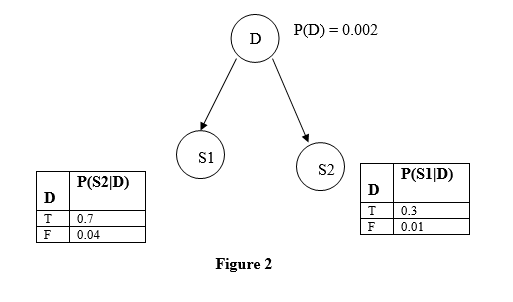
\includegraphics[width=80mm]{q6.png}
\end{figure}

\[P(D|S1, S2)=\frac{P(D, S1, S2)}{P(S1, S2)}\]

Solving the Denominator 
\[P(S1, S2) =P(D, S1, S2) + P(\sim D, S1, S2)\]\\

\\
\[ P(D,S1,S2)=P(D) \times P(S1|D) \times P(S2|D)\]
\[P(\sim D, S1, S2)=P(\sim D) \times P(S1|\sim D) \times P(S2|\sim D)\]

Inserting values into equations

\[ P(D,S1,S2)=0.002 \times 0.3 \times 0.7= 4.2 \times 10^{-4} = 0.00042\]
\[P(\sim D, S1, S2) = (1-0.002) \times 0.01 \times 0.04 = 3.992 \times 10^{-4}= 0.0003992 \]
	
		 original Equation
		\[P(D|S1, S2)=\frac{P(D, S1, S2)}{P(S1, S2)}\]
		hence 
		
	\[P(D|S1, S2)=\frac{P(D, S1, S2)}{P(D,S1,S2)+P(\sim D,S1,S2)}\] \\
		\[P(D|S1, S2)=\frac{P(D, S1, S2)}{P(D) \times P(S1|D) \times P(S2|D)+P(\sim D) \times P(S1|\sim D) \times P(S2|\sim D)}\]\\

	values are inserted into equation
		\[P(D|S1, S2)=\frac{0.002 \times 0.3 \times 0.7}{(0.002 \times 0.3 \times 0.7)+((1-0.002) \times 0.01 \times 0.04)}=\frac{4.2 \times 10^{-4}}{8.192 \times 10^{-4}}= \frac{0.00042}{0.0008192}\]
	
\[P(D|S1, S2)=5.1269 \times 10^{-1}= 0.51269\]
	
	\section{Date}
	\date{\today}
	
	

	

	
	
\end{document}

